\documentclass[9pt,twocolumn,twoside,lineno]{pnas-new}
% Use the lineno option to display guide line numbers if required.

\templatetype{pnasresearcharticle} % Choose template 
% {pnasresearcharticle} = Template for a two-column research article
% {pnasmathematics} %= Template for a one-column mathematics article
% {pnasinvited} %= Template for a PNAS invited submission

\title{Orbital-use fees could more than quadruple the value of the space industry}

% Use letters for affiliations, numbers to show equal authorship (if applicable) and to indicate the corresponding author
\author[a]{Akhil Rao}
\author[b,c,d]{Matthew Burgess} 
\author[d]{Daniel Kaffine}

\affil[a]{Department of Economics, Middlebury College}
\affil[b]{Cooperative Institute for Research in Environmental Sciences, University of Colorado Boulder}
\affil[c]{Environmental Studies Program, University of Colorado Boulder}
\affil[d]{Department of Economics, University of Colorado Boulder}

% Please give the surname of the lead author for the running footer
\leadauthor{Rao} 

% Please add here a significance statement to explain the relevance of your work
\significancestatement{Authors must submit a 120-word maximum statement about the significance of their research paper written at a level understandable to an undergraduate educated scientist outside their field of speciality. The primary goal of the Significance Statement is to explain the relevance of the work in broad context to a broad readership. The Significance Statement appears in the paper itself and is required for all research papers.}

% Please include corresponding author, author contribution and author declaration information
\authorcontributions{A.R. and D.K. conceived the project; A.R. performed the analysis, with input from M.G.B. and D.K.; A.R., M.G.B., and D.K. wrote the paper.}
\authordeclaration{The authors have no competing interests.}
%\equalauthors{\textsuperscript{1}A.O.(Author One) contributed equally to this work with A.T. (Author Two) (remove if not applicable).}
\correspondingauthor{\textsuperscript{2}To whom correspondence should be addressed. E-mail: akhilr@middlebury.edu}

% At least three keywords are required at submission. Please provide two to five keywords, separated by the pipe symbol.
\keywords{Keyword 1 $|$ Keyword 2 $|$ Keyword 3 $|$ ...} 

\begin{abstract}
The space industry’s rapid recent growth represents the latest example of the Tragedy of the Commons1,2. Satellites launched into orbit contribute to—and risk damage from—a growing buildup of space debris and other satellites. Collision risk from this orbital congestion is costly to satellite operators1. Technological and managerial solutions—such as active debris removal or end-of-life satellite deorbit guidelines—are currently being explored by space regulatory authorities3,4. However, none of these approaches address the underlying incentive problem: satellite operators do not account for the costs they impose on each other via collision risk. \\

Here, we show that an internationally harmonized orbital-use fee can correct these incentives and substantially increase the value of the space industry. We construct and analyze a model of commercial launches and debris accumulation in low-Earth orbit. Our model projects that the economically optimal fee starts at roughly \$13,500 dollars per satellite per year in 2020, and gradually increases thereafter, similar to carbon taxes. The long-run value of the satellite industry would more than quadruple by 2040—increasing from around \$600 billion under business-as-usual to around \$3 trillion. In contrast, we project that purely technological solutions, such as debris removal, are unlikely to fully address the problem of orbital congestion. In some cases, our model finds that debris removal worsens economic damages from congestion by increasing launch incentives. In other sectors, addressing the Tragedy of the Commons has often been a game of catch-up, with substantial social costs5. In the infant space industry, there is a rare opportunity to get out ahead, if the right incentives can be put in place.
\end{abstract}

\dates{This manuscript was compiled on \today}
\doi{\url{www.pnas.org/cgi/doi/10.1073/pnas.XXXXXXXXXX}}

\begin{document}

\maketitle
\thispagestyle{firststyle}
\ifthenelse{\boolean{shortarticle}}{\ifthenelse{\boolean{singlecolumn}}{\abscontentformatted}{\abscontent}}{}

% If your first paragraph (i.e. with the \dropcap) contains a list environment (quote, quotation, theorem, definition, enumerate, itemize...), the line after the list may have some extra indentation. If this is the case, add \parshape=0 to the end of the list environment.
\dropcap{I}n 2017, 466 new satellites were launched—more than double the previous year’s launches, and more than 20\% of all active satellites in orbit in 20176,7. Rapid space industry growth is projected to continue, driven largely by commercial satellites (Fig. 1). This growth is driving buildup of debris in low-Earth orbit, currently including over 15,000 objects1. Collision risk from debris is costly; collisions damage or destroy expensive capital assets that are difficult or impossible to repair. Debris buildup could eventually make some low-Earth orbits economically unviable and other orbits difficult or impossible to access8. In the worst case—though uncertain and occurring over long time horizons—debris growth could become self-sustaining due to collisions between debris objects, a tipping point called Kessler Syndrome8,9. 

Proposed solutions have so far largely been technological and managerial, aimed at mapping, avoiding, and removing debris3,4. These include end-of-life deorbit guidelines and “keep-out” zones for active satellites, and nets, harpoons and lasers to deorbit debris4. However, with open access to orbits, reducing debris and collision risk incentivizes additional satellite launches, which eventually restores the debris and risk. For instance, if firms were willing to tolerate a 0.1\% annual risk of satellite loss before a technological improvement in debris removal, they will be willing to launch more satellites until the 0.1\% annual risk of satellite loss is restored. 

Thus, the core of the space debris problem is incentives, not technology. Since satellite operators are unable to secure exclusive property rights to their orbital paths or recover collision-related costs imposed by others, prospective operators face a choice between launching profitable satellites, thereby imposing current and future collision risk on others, or not launching and leaving those profits to competitors.  This is a classic Tragedy of the Commons problem, as others have noted1,6,10,11. It can be economically efficiently addressed via incentive-based solutions, such as fees or tradable permits for time in orbit, analogous to carbon taxes or cap-and-trade12. Incentives should target objects in orbit—rather than launches—because orbiting objects are what directly impose collision risk on other satellites13. We provide the first analysis, to our knowledge, quantifying the economic benefits of implementing such incentives. 

We use a model combining rich physical dynamics with satellite economics to quantify the benefits of an internationally harmonized ‘orbital-use fee’ (OUF) relative to a business-as-usual (BAU) open-access scenario, and a scenario with active debris removal, while accounting for the effects of each scenario on satellite launch decisions (see Methods and Supplementary Methods). While we focus on an orbital-use fee for analytical convenience, it is conceptually equivalent to other mechanisms for pricing orbits, such as tradable permits.

Our physical model of satellite and debris evolution in orbit obeys the relevant accounting identities and utilizes reduced-form approximations of physical processes validated in other works14,15. We fit and calibrate the model using data on collision risk and orbital debris produced by the European Space Agency (ESA)16, and data on active satellites from the Union of Concerned Scientists (UCS)7 (see Methods and Supplementary Methods), with the ESA dataset covering 1958-2017 and the UCS dataset covering 1957-2017. By assumption, runaway debris growth (Kessler Syndrome) cannot occur in our physical model, which likely makes it understate the benefits of OUFs (see Methods). Our economic model assumes satellites are launched and operated to maximize per-satellite private profits, net of any fees, subject to collision risk. We calibrate the model by fitting the BAU scenario (no fees or debris removal) to historical industry data and launch trends6,7 (see Methods and Supplementary Methods). 

We project future launch rates to 2040 under the BAU scenario using our fitted model and published projections of future growth of the space economy17. We then calculate launch rates that would maximize the long-run value of the industry, and we calculate the time series of OUFs that would incentivize these optimal launch rates. The industry value is measured as net present value (NPV)—the long-run value of the entire fleet of satellites in orbit, accounting for both the financial costs of replacing satellites due to natural retirement and collisions, as well as the opportunity cost of investing funds in satellites rather than capital markets. For instance, an NPV of \$1 trillion in 2020 means that the sum total of the stream of net benefits, looking into the future from 2020 and accounting for the timing of the net benefits, is \$1 trillion.

Though our models are deliberately simplified for tractability, they are based on previously-validated approaches to orbital object modeling14,15, and our calibrations allow us to reproduce observed trends and magnitudes in the growth of orbital debris and satellite stocks, as well as the calculated collision risk (see Extended Data Fig. 2). Nonetheless, our projections should be interpreted as order-of-magnitude approximations that can be refined as needed by more detailed models. In these respects, our approach mirrors integrated assessment modeling approaches that have been useful in developing solutions to other natural resource management problems (e.g., ref 18).  

We project that shifting from open access to the optimal series of OUFs in 2020 would increase the NPV of the satellite industry from around \$600 billion under business-as-usual to around \$3 trillion—a more than four-fold increase (Fig. 2) (4.68 to 6.54 times in 95\% of parameter sets randomly drawn from their calibrated distributions; see Extended Data figure 10b and Supplementary Methods). Assuming a 5\% market rate of return, an increase of \$2.5 trillion in NPV would be equivalent to annual benefits of approximately \$120 billion in perpetuity. Based on our calculations (see Methods), the optimal OUF starts at roughly \$13,500 per satellite per year in 2020 and escalates at $\sim$14.8\% per year to around \$244,000 per satellite per year in 2040. Rising optimal price paths are common in environmental pricing such as carbon taxes12. The rising price path in this case partly reflects the rising value of safer orbits (resulting in rising industry NPV; see Fig. 2a) created by the OUF.

Forgone NPV from the satellite industry in 2040—the cost of inaction under BAU—escalates from around \$300 billion if optimal management begins in 2025 to around \$750 billion if optimal management begins in 2035. Without OUFs, losses remain substantial even when active debris removal is available. In a best-case analysis where we assume debris removal is costless (i.e., it is provided for free, and requires no additional satellites to implement), debris removal can only recover up to 8.6\% of the value lost under open access. At worst, debris-removal can exacerbate orbital congestion via a rebound-type effect, causing additional losses on the order of 1.8\% of the value already lost from open access (see Extended Data Fig. 5 and Supplementary Discussion). The inability of debris removal to induce efficient orbit use is driven by open-access launching behavior and underscores the importance of policies to correct economic incentives to launch satellites.

Escalating costs of inaction is a common feature of the Tragedy of the Commons, evident in several other sectors in which it went unaddressed for long periods of time5. For example, tens of billions of dollars in net benefits are lost annually from open-access or poorly-managed fisheries around the globe19. Similarly, open access to oil fields in U.S. at the turn of the century drove recovery rates down to 20-25\% at competitively drilled sites, compared to 85-90\% potential recovery under optimal management20. Open access to roadways—somewhat analogous to orbits—is estimated to create traffic congestion costs in excess of \$120 billion a year in the U.S. alone21. In contrast, there is a rare opportunity to get out ahead of the Tragedy of the Commons in the young space industry.

The international and geopolitically complex nature of the space sector poses challenges to implementing orbital-use pricing systems, which need not be insurmountable. Theory suggests countries could each collect and spend orbital-use fee revenues domestically, without losing economic efficiency, as long as the fee’s magnitude was internationally harmonized22. An example of such a system is the Vessel Day Scheme (VDS) used by the Parties to the Nauru Agreement (PNA) to manage tuna fisheries. Under the VDS, PNA countries each lease fishing rights within their waters, using a common price floor23. The European Union’s (E.U.) Emissions Trading System (ETS) provides an example of an internationally coordinated tradable permit system24. Notably, each of these pricing programs is built on a pre-existing international governance institution (the Nauru Agreement and the E.U.). 

An OUF could also be built within existing space governance institutions, such as the Outer Space Treaty25. For example, Article VI states that countries supervise their space industries, which provides a framework for orbital-use fees to be administered nationally. Article II prohibits national appropriation of outer space, but it does not prohibit private property rights, thus potentially allowing for tradable orbital permitting.

Military and other non-commercial uses of satellites are also important to consider in designing any incentive-based orbital management policy. In December of 2018, 430 of 1957 satellites in orbit had acknowledged military users7. Some ostensibly-commercial satellites may also fill national security needs. Further, governments provide satellite-based public goods to their citizens, such as remote sensing and GIS. In addition to collision risk, satellite and debris buildup may impose costly interference on ground-based space observation systems. OUFs targeting the commercial sector should account for these interests and monitor, as best possible, any "leakage" (see ref 26) from the commercial sector to the government sector. Antarctica and the Arctic Circle offer two models of internationally managed regions in which commercial interests, environmental interests, and geopolitical interests interact (e.g., ref 27).

Despite the simplifying assumptions of our model, its key qualitative results may be robust to geopolitical and other complexities. Experience in other resource contexts supports our projection that technological or managerial solutions to the space debris problem are unlikely to be as effective as incentive-based solutions. For instance, in fisheries, attempts to restrict entry have led to “capital stuffing,” where existing vessels heavily invest in harvest capacity28. Similarly, catch limits led to the “race to fish” phenomena29, whereby fishermen exert extreme effort to harvest as much as possible before the catch limit is reached. Attempts to build new highway capacity to reduce traffic congestion have been frustrated because new capacity induces new demand for travel30. By contrast, policies such as individual tradable quotas31 and congestion charges32 directly target the underlying incentive issue and have proven more successful, though are not without some controversy due to distributional effects33.

The Tragedy of the Space Commons is an international incentives problem and therefore needs an internationally coordinated incentive-based solution. Our analysis suggests such solutions could add trillions in value to the industry. Programs such as the EU Emissions Trading System and the PNA’s Vessel Day Scheme offer potential models for success.

%Note: please start your introduction without including the word ``Introduction'' as a section heading (except for math articles in the Physical Sciences section); this heading is implied in the first paragraphs. 

%\section*{Guide to using this template on Overleaf}
%
%Please note that whilst this template provides a preview of the typeset manuscript for submission, to help in this preparation, it will not necessarily be the final publication layout. For more detailed information please see the \href{http://www.pnas.org/site/authors/format.xhtml}{PNAS Information for Authors}.
%
%If you have a question while using this template on Overleaf, please use the help menu (``?'') on the top bar to search for \href{https://www.overleaf.com/help}{help and tutorials}. You can also \href{https://www.overleaf.com/contact}{contact the Overleaf support team} at any time with specific questions about your manuscript or feedback on the template.

\subsection*{Author Affiliations}

Include department, institution, and complete address, with the ZIP/postal code, for each author. Use lower case letters to match authors with institutions, as shown in the example. Authors with an ORCID ID may supply this information at submission.

%\subsection*{Submitting Manuscripts}
%
%All authors must submit their articles at \href{http://www.pnascentral.org/cgi-bin/main.plex}{PNAScentral}. If you are using Overleaf to write your article, you can use the ``Submit to PNAS'' option in the top bar of the editor window. 

%\subsection*{Format}
%
%Many authors find it useful to organize their manuscripts with the following order of sections;  Title, Author Affiliation, Keywords, Abstract, Significance Statement, Results, Discussion, Materials and methods, Acknowledgments, and References. Other orders and headings are permitted.

%\subsection*{Manuscript Length}
%
%A standard 6-page article is approximately 4,000 words, 50 references, and 4 medium-size graphical elements (i.e., figures and tables). The preferred length of articles remains at 6 pages, but PNAS will allow articles up to a maximum of 12 pages.

%\subsection*{References}
%
%References should be cited in numerical order as they appear in text; this will be done automatically via bibtex, e.g. \cite{belkin2002using} and \cite{berard1994embedding,coifman2005geometric}. All references cited in the main text should be included in the main manuscript file.

%\subsection*{Data Archival}
%
%PNAS must be able to archive the data essential to a published article. Where such archiving is not possible, deposition of data in public databases, such as GenBank, ArrayExpress, Protein Data Bank, Unidata, and others outlined in the Information for Authors, is acceptable.
%
%\subsection*{Language-Editing Services}
%Prior to submission, authors who believe their manuscripts would benefit from professional editing are encouraged to use a language-editing service (see list at www.pnas.org/site/authors/language-editing.xhtml). PNAS does not take responsibility for or endorse these services, and their use has no bearing on acceptance of a manuscript for publication. 

\begin{figure}%[tbhp]
\centering
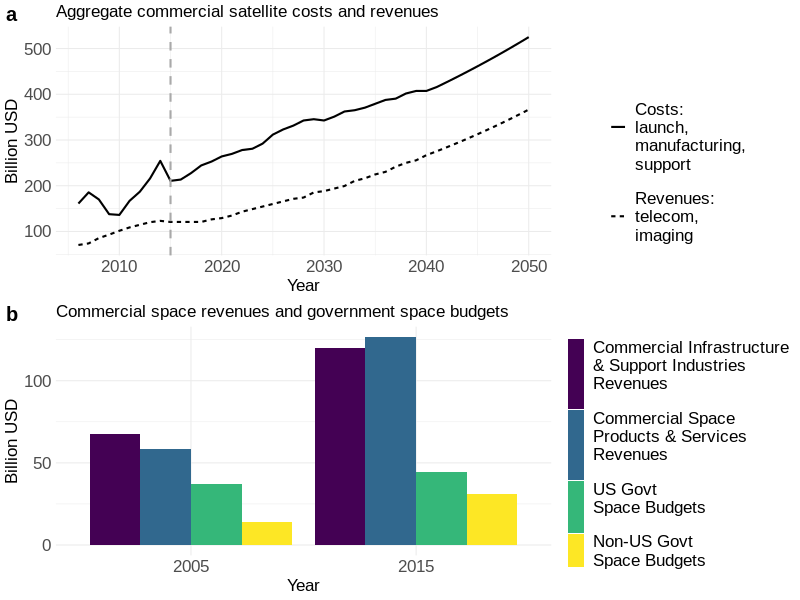
\includegraphics[width=.8\linewidth]{main_text_figure_1.png}
\caption{State of the industry (data from refs. 6, 7, 17). a: Projected growth of satellite industry costs and revenues.  Revenues and costs are yearly flows.  Costs are not annuitized over the satellite lifetime. b: Observed growth in commercial space sector revenues and government space budgets.}
\label{fig:MT1}
\end{figure}

\begin{figure}%[tbhp]
	\centering
	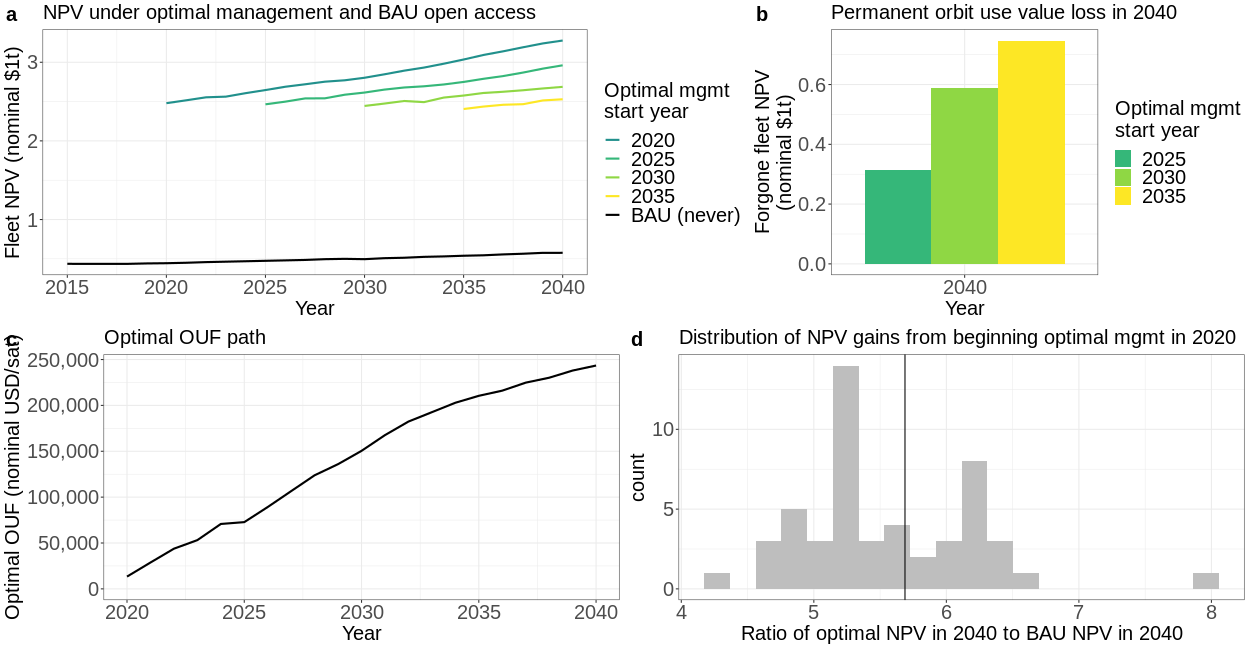
\includegraphics[width=.8\linewidth]{main_text_figure_2.png}
	\caption{Projected gains from optimal management via orbital-use fees. a: NPV of orbit recovery, with optimal management beginning in different years. BAU is shown in black. The NPV gain is the difference between optimal management and BAU. b: Loss in permanent orbit use value from delaying optimal management, relative to 2020 optimal management start. c: Time path of the optimal OUF. d: Distribution of the ratio of optimal NPV in 2040 (assuming optimal management begins in 2020) to BAU NPV in 2040 using 50 draws of alternate parameter sets. The distribution is calculated via a residual-bootstrap resampling procedure which illustrates the effect of calibration uncertainty. We describe the bootstrap in more detail in section 1.4 of the Supporting Information.}
	\label{fig:MT2}
\end{figure}

%\begin{SCfigure*}[\sidecaptionrelwidth][t]
%\centering
%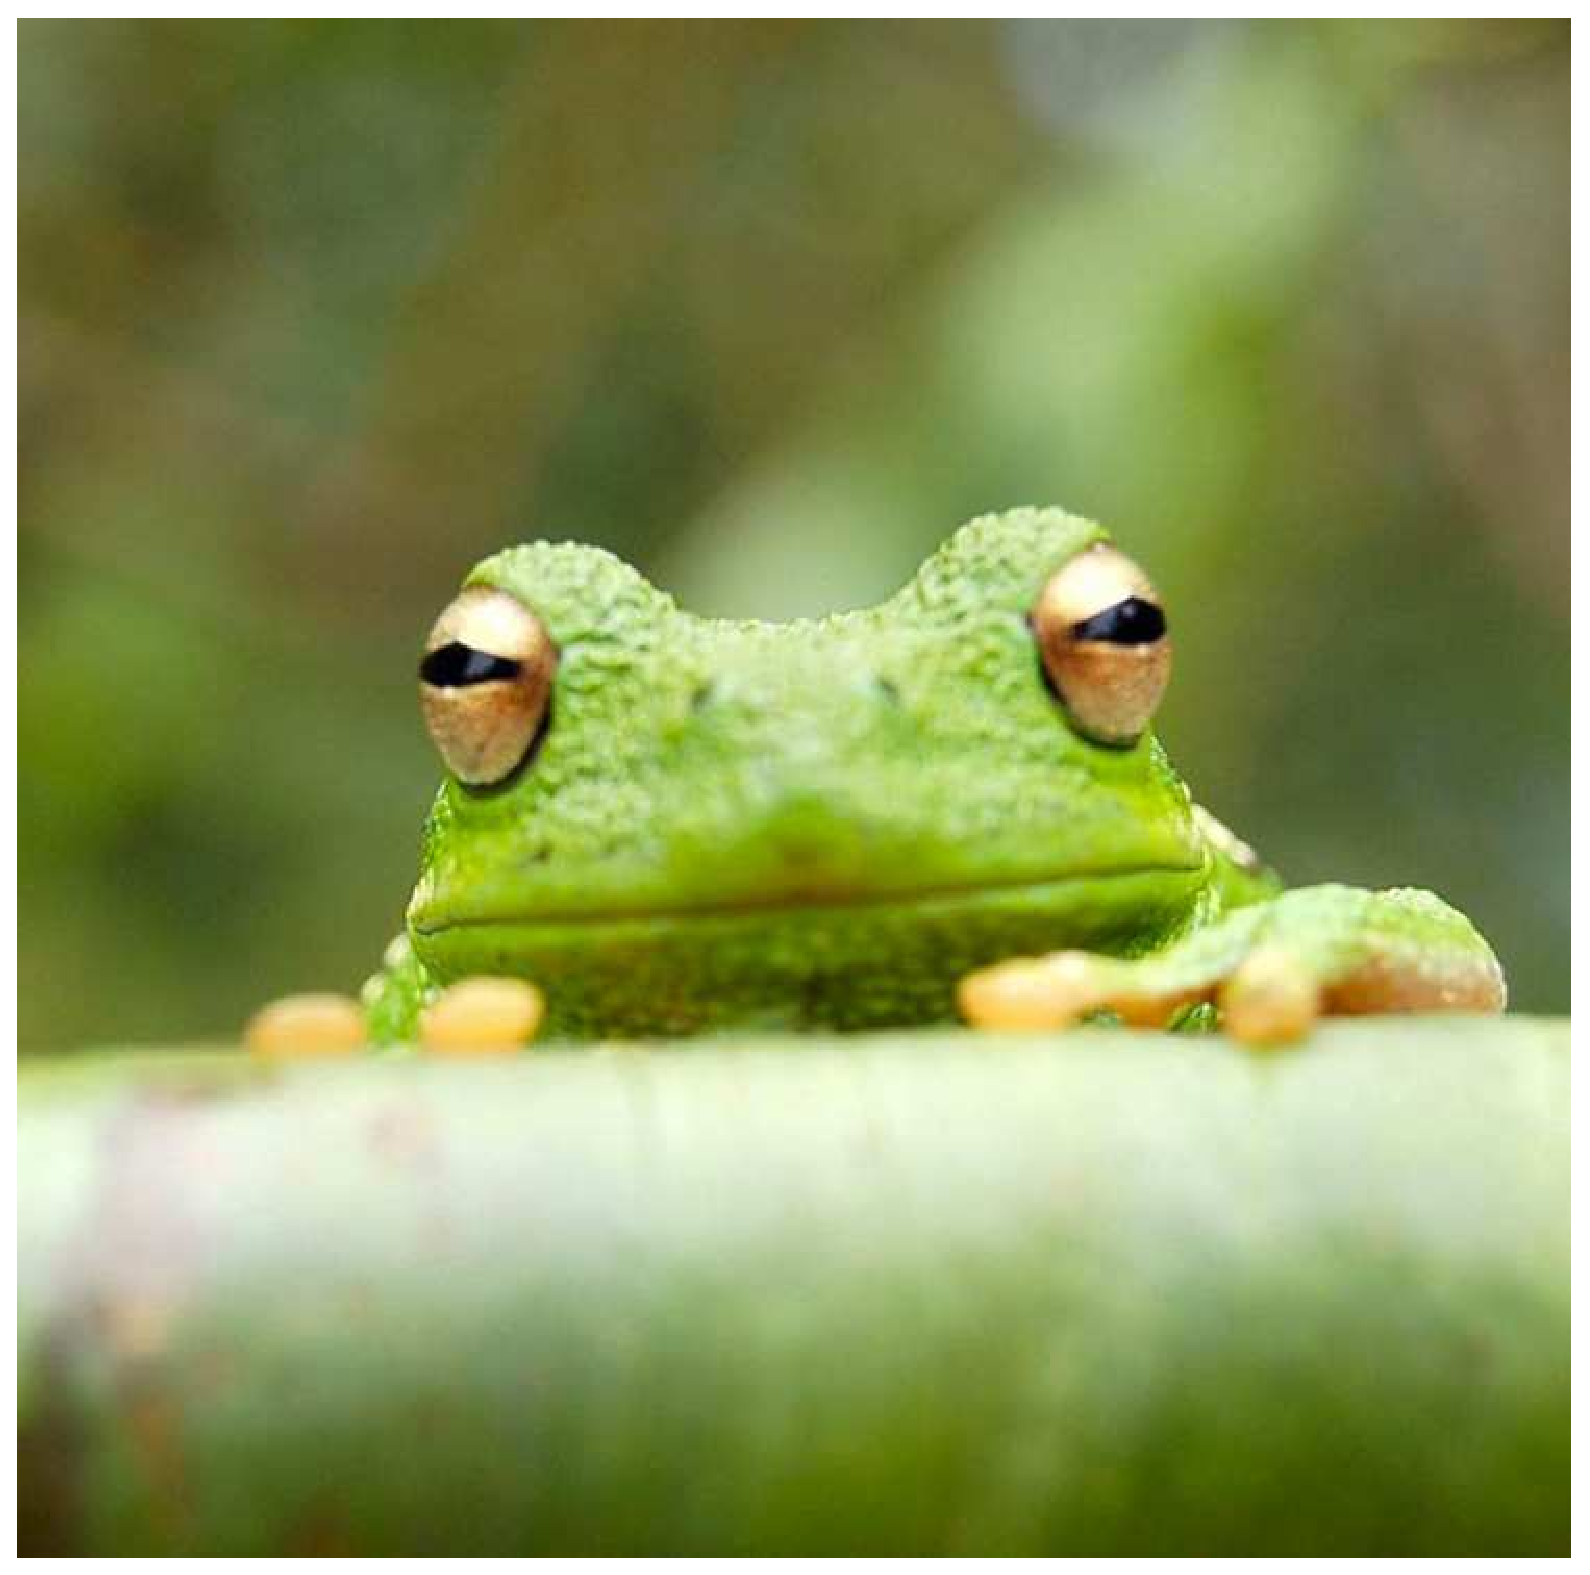
\includegraphics[width=11.4cm,height=11.4cm]{frog}
%\caption{This caption would be placed at the side of the figure, rather than below it.}\label{fig:side}
%\end{SCfigure*}

\subsection*{Digital Figures}

EPS, high-resolution PDF, and PowerPoint are preferred formats for figures that will be used in the main manuscript. Authors may submit PRC or U3D files for 3D images; these must be accompanied by 2D representations in TIFF, EPS, or high-resolution PDF format. Color images must be in RGB (red, green, blue) mode. Include the font files for any text.

Images must be provided at final size, preferably 1 column width (8.7cm). Figures wider than 1 column should be sized to 11.4cm or 17.8cm wide. Numbers, letters, and symbols should be no smaller than 6 points (2mm) and no larger than 12 points (6mm) after reduction and must be consistent. 

Figures and Tables should be labelled and referenced in the standard way using the \verb|\label{}| and \verb|\ref{}| commands.

Figure \ref{fig:frog} shows an example of how to insert a column-wide figure. To insert a figure wider than one column, please use the \verb|\begin{figure*}...\end{figure*}| environment. Figures wider than one column should be sized to 11.4 cm or 17.8 cm wide. Use \verb|\begin{SCfigure*}...\end{SCfigure*}| for a wide figure with side captions.

\subsection*{Tables}
Tables should be included in the main manuscript file and should not be uploaded separately.

%\subsection*{Single column equations}
%
%Authors may use 1- or 2-column equations in their article, according to their preference.
%
%To allow an equation to span both columns, use the \verb|\begin{figure*}...\end{figure*}| environment mentioned above for figures.
%
%Note that the use of the \verb|widetext| environment for equations is not recommended, and should not be used. 
%
%\begin{figure*}[bt!]
%\begin{align*}
%(x+y)^3&=(x+y)(x+y)^2\\
%       &=(x+y)(x^2+2xy+y^2) \numberthis \label{eqn:example} \\
%       &=x^3+3x^2y+3xy^3+x^3. 
%\end{align*}
%\end{figure*}
%
%
%\begin{table}%[tbhp]
%\centering
%\caption{Comparison of the fitted potential energy surfaces and ab initio benchmark electronic energy calculations}
%\begin{tabular}{lrrr}
%Species & CBS & CV & G3 \\
%\midrule
%1. Acetaldehyde & 0.0 & 0.0 & 0.0 \\
%2. Vinyl alcohol & 9.1 & 9.6 & 13.5 \\
%3. Hydroxyethylidene & 50.8 & 51.2 & 54.0\\
%\bottomrule
%\end{tabular}
%
%\addtabletext{nomenclature for the TSs refers to the numbered species in the table.}
%\end{table}

%\subsection*{Supporting Information Appendix (SI)}
%
%Authors should submit SI as a single separate SI Appendix PDF file, combining all text, figures, tables, movie legends, and SI references. PNAS will publish SI uncomposed, as the authors have provided it. Additional details can be found here: \href{https://www.pnas.org/page/authors/format#Supporting_Information}{policy on SI}. The PNAS Overleaf SI template can be found \href{https://www.overleaf.com/latex/templates/pnas-template-for-supplementary-information/wqfsfqwyjtsd}{here}. Refer to the SI Appendix in the manuscript at an appropriate point in the text. Number supporting figures and tables starting with S1, S2, etc.
%
%Authors who place detailed materials and methods in an SI Appendix must provide sufficient detail in the main text methods to enable a reader to follow the logic of the procedures and results and also must reference the SI methods. If a paper is fundamentally a study of a new method or technique, then the methods must be described completely in the main text.

\subsubsection*{SI Datasets} 
%
%Supply .xlsx, .csv, .txt, .rtf, or .pdf files. This file type will be published in raw format and will not be edited or composed.

%
%\subsubsection*{SI Movies}
%
%Supply Audio Video Interleave (avi), Quicktime (mov), Windows Media (wmv), animated GIF (gif), or MPEG files. Movie Legends should be included in the SI Appendix file. All movies should be submitted at the desired reproduction size and length. Movies should be no more than 10 MB in size.
%
%
%\subsubsection*{3D Figures}
%
%Supply a composable U3D or PRC file so that it may be edited and composed. Authors may submit a PDF file but please note it will be published in raw format and will not be edited or composed.
%

\matmethods{
	Here we describe the data sources, calibration procedures, and dynamic optimization model used to quantify the economic benefits of orbits under BAU and under optimal management via an OUF.
	
	\subsection*{Data} 
	We use data on collision risk, orbital debris counts, and satellite counts provided by the European Space Agency (ESA)16 and the Union of Concerned Scientists (UCS)7 to calibrate our physical models of aggregate active satellite and debris evolution. We calibrate our economic model of open access launching using historical aggregate returns and costs for the space industry obtained from ref. 6 and launch data calculated from ref. 7. Our physical data cover 1957–2017, while our historical economic data cover 2005–2015. 
	
	For each year, the ESA data provides counts of the number of debris objects in orbit within a specified 50 km. altitude band (average orbital altitude) beginning at 100 km. above mean sea level and extending to 2000 km. above sea level, as well as the estimated probability that a collision occurs in the same bands. Each observation in the ESA data corresponds to a year, and each column corresponds to an altitude band. The UCS data describe all known active satellites currently in orbit, including variables for stated purpose, date of launch, and date of deorbit (if applicable). Each observation in this dataset corresponds to an active satellite, with corresponding variables describing that satellite. This dataset is spread over a series of files, released at roughly quarterly to semi-annually frequencies between 2005–2018, from which we reconstruct yearly counts of the number of active satellites in the 100-2000 km. range from 1957–2015. 
	
	The economic dataset we use comes from refs. 6 and 17, with data from ref. 6 representing historical data. An observation in the original dataset represents a year, with variables for dollars spent on different space sector activities, e.g. satellite construction and launch services, ground observation services, government spending by different national governments, etc. We classify these entries into yearly revenues flowing to satellite owners, and yearly costs of building, launching, and operating satellites (which we refer to as “launch costs” for brevity). We merge these data with the estimated collision probability data from the ESA dataset16.
	
	An observation in the final, merged dataset we use for physical model calibration represents a year in 1957–2015, which includes variables for active satellite count, debris count, estimated collision probability, and estimated returns to and costs of launching a satellite in the 100-2000 km. range.  An observation in the final, merged dataset we use for economic model calibration represents a year in 2005–2015, with variables for aggregate satellite sector revenues and costs, the yearly gross rate of return on a satellite, the year-over-year change in launch costs, and the estimated collision probability. We describe our data and variable construction procedures in greater detail in Supplementary Methods.
	
	\subsection*{Calibrating the physical model} 
	We construct the laws of motion for aggregate active satellite and debris stocks from accounting relationships. We assume that a) a constant fraction (3.3%) of undestroyed active satellites naturally deorbit each period (without creating additional debris), b) a constant fraction (49%) of debris deorbits each period, and c) new fragment creation occurs due to launch debris, anti-satellite missile tests, and collisions between orbital objects. We parameterize the probability that an active satellite is destroyed in a collision using an approximate form validated in other works14,15, and from that functional form derive an expression for the number of new fragments created in collisions. The parameters in these functions are calibrated separately. Specific formulas are presented in Supplementary Methods.
	
	We first calibrate the collision probability function by fitting it to data on the estimated probability of a collision between 100-2000 km provided by ESA, using constrained nonlinear least squares. We constrain the parameter estimates to be positive, which is consistent with the physical interpretation of the collision probability parameters as combinations of positive values: the magnitude of velocity differences between colliding objects, the total cross-sectional area of the collision, and scaling values that relate object counts to object densities.
	
	We then calibrate the debris law of motion, using the estimated collision probability parameters, by constrained ridge regression. We use ridge regression to improve the debris model fit, given that we have relatively few observations for the number of parameters. We constrain the parameters to comply with their physical interpretations: parameters representing numbers of fragments created in collisions must be positive, while the debris decay rate must be between 0 and 1. Given the uncertainties involved in modeling and calibrating the potential for Kessler Syndrome, we disallow the possibility of debris objects colliding with each other. This likely makes our conclusions conservative, as it likely understates the growth in collision risk over time due to debris-debris collisions. Consequently, the estimated optimal OUF is likely less than what a model with debris-debris collisions would predict, as are our estimated benefits of implementing the OUF.
	
	Finally, we calibrate the fraction of active satellites that naturally deorbit by fitting the active satellite law of motion using ordinary least squares. This yields an estimated average lifespan of approximately 30 years (the 3.3% deorbit rate mentioned above), which is consistent with an average mission length of 5 years followed by compliance with the IADC’s 25-year deorbit guideline34. We assume full compliance with the guideline to be conservative in our estimates of debris production. We describe our physical calibration procedures in greater detail in Supplementary Methods.  We show sensitivity analyses of our calibrations in Extended Data Fig. 7, and of our model projections in Extended Data Figs. 8-10. We describe our sensitivity analysis procedure in Supplementary Methods.
	
	\subsection*{Calibrating the economic model} Economic theory predicts that the collision probability will be determined by the excess rate of return on an active satellite13. However, the excess rate of return includes the internal rate of return on a satellite asset, which we do not observe, as well as factors relating to the economic structure of the various satellite-using industries involved, which we do not model. To account for these issues, we model the excess rate of return using observed aggregate revenues and costs for the satellite industry, and then include the various unknown and unmodeled factors as parameters to estimate. We then fit this model to the estimated collision probability data using ordinary least squares. Since the signs of the parameters representing the unknown and unmodeled factors are ambiguous, we do not constrain the estimates. The estimated parameters are incorporated into the economic model and used to adjust for unmodeled economic factors. The adjustment produces estimated “implied aggregate costs”, shown in Extended Data Table 3. We describe this adjustment procedure in Supplementary Methods and discuss the relevant unmodeled factors in Supplementary Discussion. We assume a market discount rate of 5 percent35. The economic gains from an OUF would be even larger in magnitude at lower social discount rates.
	
	\subsection*{Projecting open access and optimal launch rates} To project the launch rates under BAU and optimal management via an OUF, we solve the dynamic optimization problems associated with launching new satellites.  Under open access BAU, each firm wishes to maximize their own lifetime satellite profits, and the optimization problem determines each firm’s decision of whether to launch or not, which in turn determines the total launch rate across all firms. This involves calculating whether the expected lifetime revenues from another satellite exceed the cost of launching it and aggregating up from the individual decisions to the total launch rate. Under optimal management, the optimization problem directly determines the total launch rate which maximizes the NPV of the satellite fleet. This involves calculating whether the expected lifetime revenues from another satellite exceed the total industry-wide costs of launching it, including the expected costs of replacing other satellites lost due to collision risk created by the new satellite and its associated debris.
	
	Solving these dynamic optimization problems yields “launch policy functions”, which map the possible orbital states – satellite and debris counts, given current revenues and costs – into an annual launch rate. As the launch policy functions encode behavioral and institutional assumptions, the launch rates they generate are more realistic approximations of orbit management behavior than simple sensitivity analyses over all possible launch rates.  That is, the launch decisions are consistent with, and respond to changes in, economic and orbital conditions. By using the launch policy functions along with the laws of motion for the satellite and debris stocks and an initial condition, we can project the number of satellites and debris in orbit each year under a specified type of management institution. We describe the computation of the launch policy functions in more detail in Algorithms 1-3 in Supplementary Methods. 
	
	\subsection*{Calculating the optimal orbital-use fee and its benefits} To calculate the optimal OUF for each year t, we compare the expected cost of satellite-destroying collisions in year t+1 under BAU and under optimal management (see Equation 18 in Supplementary Methods). The OUF is positive whenever the optimal management solution maintains a lower collision probability than what would occur under open access BAU. The OUF is simply the marginal external cost of another satellite launch, which is the additional industry-wide cost of another satellite in orbit (additional collision risk and debris production now and in the future) that is not internalized by individual firms under BAU. By charging firms the marginal external cost of their satellite launch through an OUF, each firm’s incentives and thus their launch rates are aligned with those under industry-wide, NPV-maximizing optimal management.
	
	To calculate the benefits of imposing the OUF, we use the launch policy functions described above to compute the NPV of the entire satellite fleet under BAU and optimal management. These NPVs reflect the value of the entire satellite fleet, in perpetuity, assuming society stays on the BAU or optimal management path. The difference between the NPVs yields the gains from implementing the optimal OUF and moving from BAU to the optimal management path.
	
	Although we abstract from many of the economic and physical complications in modeling orbit use, we consider how those factors would affect our analysis in the Supplementary Methods and Supplementary Discussion. In particular, Supplementary Methods details our sensitivity analyses with respect to physical parameter uncertainty, and Supplementary Discussion considers how these concerns may impact our conclusions. Our conclusions are likely robust to the complications we abstract from, with our calculated optimal OUF and the NPV benefits of implementing it providing the correct order of magnitude with the correct qualitative features. Future research will improve our estimates and provide more detailed guidance to policymakers.
}

\showmatmethods{} % Display the Materials and Methods section

\acknow{We acknowledge funding from the University of Colorado Boulder. We thank Francesca Letizia of the European Space Agency for data on debris fragments and collision risk in low-Earth orbit, and Teri Grimwood of the Union of Concerned Scientists for the full catalog of UCS active satellite data. We thank Waleed Abdalati for helpful comments on a previous draft, and attendees of a European Space Agency Space Debris Office seminar for providing helpful feedback on our results.}

\showacknow{} % Display the acknowledgments section

% Bibliography
\bibliography{../memos/database}

\end{document}